% !TEX TS-program = pdflatexmk
\documentclass{article}
\usepackage[a4paper, margin=1in]{geometry}
\usepackage{graphicx}
\usepackage{epstopdf}
\usepackage{float}
\usepackage[numbers]{natbib}
\usepackage{lineno}
\usepackage{numcompress}
\usepackage{amssymb}
\usepackage{hyperref}
\usepackage{setspace}
\usepackage{authblk}
\def\UrlBreaks{\do\/\do-}

\modulolinenumbers[5]
\graphicspath{{figs/}}

\DeclareGraphicsRule{.tif}{png}{.png}{`convert #1 `dirname #1`/`basename #1 .tif`.png}

\def\vm{Vaximap}

\graphicspath{{figs/}{../analysis}{../survey}}

\begin{document}

\title{\textbf{\vm{}{}: optimal delivery of vaccinations for housebound patients}}
\author[1]{Thomas F. Kirk\thanks{corresponding author: tomfrankkirk@gmail.com}}
\author[2]{Adam J. Barker}
\author[3]{Armen Bodossian}
\author[1,4]{Robert Staruch}
\affil[1]{Institute of Biomedical Engineering, Department of Engineering Science, University of Oxford, Oxford}
\affil[2]{Squarepoint Capital LLP, London}
\affil[3]{Vodafone Group PLC, London}
\affil[4]{Defence Deanery, Academic Department of Military Surgery and Trauma, Birmingham}
\maketitle

\doublespacing
\linenumbers

\section{Abstract}

During the United Kingdom’s Covid-19 vaccination campaign, general practitioners (GPs) have held responsibility for vaccinating housebound patients. This presented them with a large, complex and unfamiliar logistical challenge, namely determining the most time-efficient route to visit multiple patients at their home address, better known as the travelling salesman problem (TSP). In response to a lack of existing solutions for the TSP tailored specifically to vaccination, and in light of overwhelming demand from GPs, Vaximap (\url{www.vaximap.org}) was created in January 2021 to automate the process of route planning. It is free of charge for all users and has been used to plan vaccinations for over 400,000 patients. This article analyses usage data to quantify the time and financial savings accrued; these are estimated at 5,300 hours of practitioner time (2.75 work-years) and £102,000 respectively. Hence, we show that the adoption of Vaximap yielded both time and cost savings for GP surgeries and accelerated the UK’s Covid-19 vaccination campaign at a critical moment.

\section{Background}
\label{sec:background}

The UK’s vaccination campaign against SARS-Cov-2 was launched in early 2021. One of the first questions to be addressed was to determine how severely limited quantities of vaccine should be allocated across the population in order to most quickly reduce the severity of disease. The Joint Committee on Vaccination and Immunisation (JCVI) identified nine priority groups of descending age and risk order \cite{JCVI2020}; the top four groups, including 3.7 million clinically extremely vulnerable individuals \cite{ONS_CEV}, were to be vaccinated by the 15th February 2021, just six weeks into the wider campaign \cite{NHSE_uplift}. Within the top four groups, it is estimated that around half a million individuals were housebound\footnote{Numerous freedom of information requests to NHS England, Public Health England and the JCVI have not yielded a precise figure. Correspondence with a member of the Health Informatics Group at the Royal College of General Practitioners suggests a figure of around 500,000 and a lower bound of 250,000.}, meaning that vaccination would need to take place at the patient’s home. Responsibility for vaccinating these patients was assigned to GPs, thus presenting primary care with a complex and unfamiliar logistical challenge of a scale wholly unprecedented in recent history. 

Even before the pandemic created additional pressures, primary care in the UK was stretched and under-resourced \cite{TheKingsFund2020, BritishMedicalAssociation2022}. There exist substantial regional variations in primary care accessibility: for example, there are around 3,000 patients per GP in Luton, compared to 1,770 per GP in the Vale of York \cite{Rolewicz2021}. The burden imposed upon GPs by the additional responsibility to plan and deliver vaccinations to housebound patients thus fell asymmetrically across primary care. Recognising that this task would stretch already-limited resources, NHS England allocated additional funding to GPs in February 2021 specifically to support the vaccination of housebound individuals and ensure the wider campaign could proceed on schedule \cite{NHSE_uplift}. Crucially, however, no specific technical support was put in place to support housebound vaccination, an issue that was raised by individual GPs on social media discussions, alongside the fact that they had not been given any training for a task that was completely new to them. In short, the funds had been allocated, but not the means. In response to these concerns from clinicians, Vaximap was created to automate the process of route planning.

The central problem in optimising the vaccination of housebound patients is determining the fastest order in which to visit the individuals. This is an example of the travelling salesman problem (TSP), which has been extensively studied in the domain of computer science. Notwithstanding numerous solutions to the problem \cite{Laporte1990}, some of which have been applied in a medical context \cite{Shao2012}, vaccination imposes an extra constraint: because there are a fixed number of doses in a vial, it is preferable sort patients into groups of this same number. This ensures that exactly one vial (or integer multiples thereof) of vaccine will be required per group of visited patients. Separately, due to the cold-storage requirements of the vaccines themselves, visiting patients in the fastest order minimises the time that vials spend outside of the cold chain. Taken together, these two factors reduce vaccine wastage, especially important given the limited availability of supplies during the early stages of the campaign \cite{NHSE_AZ}.

Vaximap is a free-to-use website (\url{www.vaximap.org}) to which a user uploads an Excel spreadsheet of patient postcodes to be visited. The patients are sorted into groups of fixed size based on proximity to each other, the fastest route within each group found, and directions with estimated travel times returned to the user (an example is shown in figure \ref{demo}). Within a month of operation, 100,000 vaccine deliveries had been planned on the site and the service was adopted for use by roving military vaccination teams during operation RESCRIPT, the UK military's support to HM Government during the pandemic. As of May 2022, over 400,000 deliveries have been planned using the service.

\begin{figure}[H]
\centering
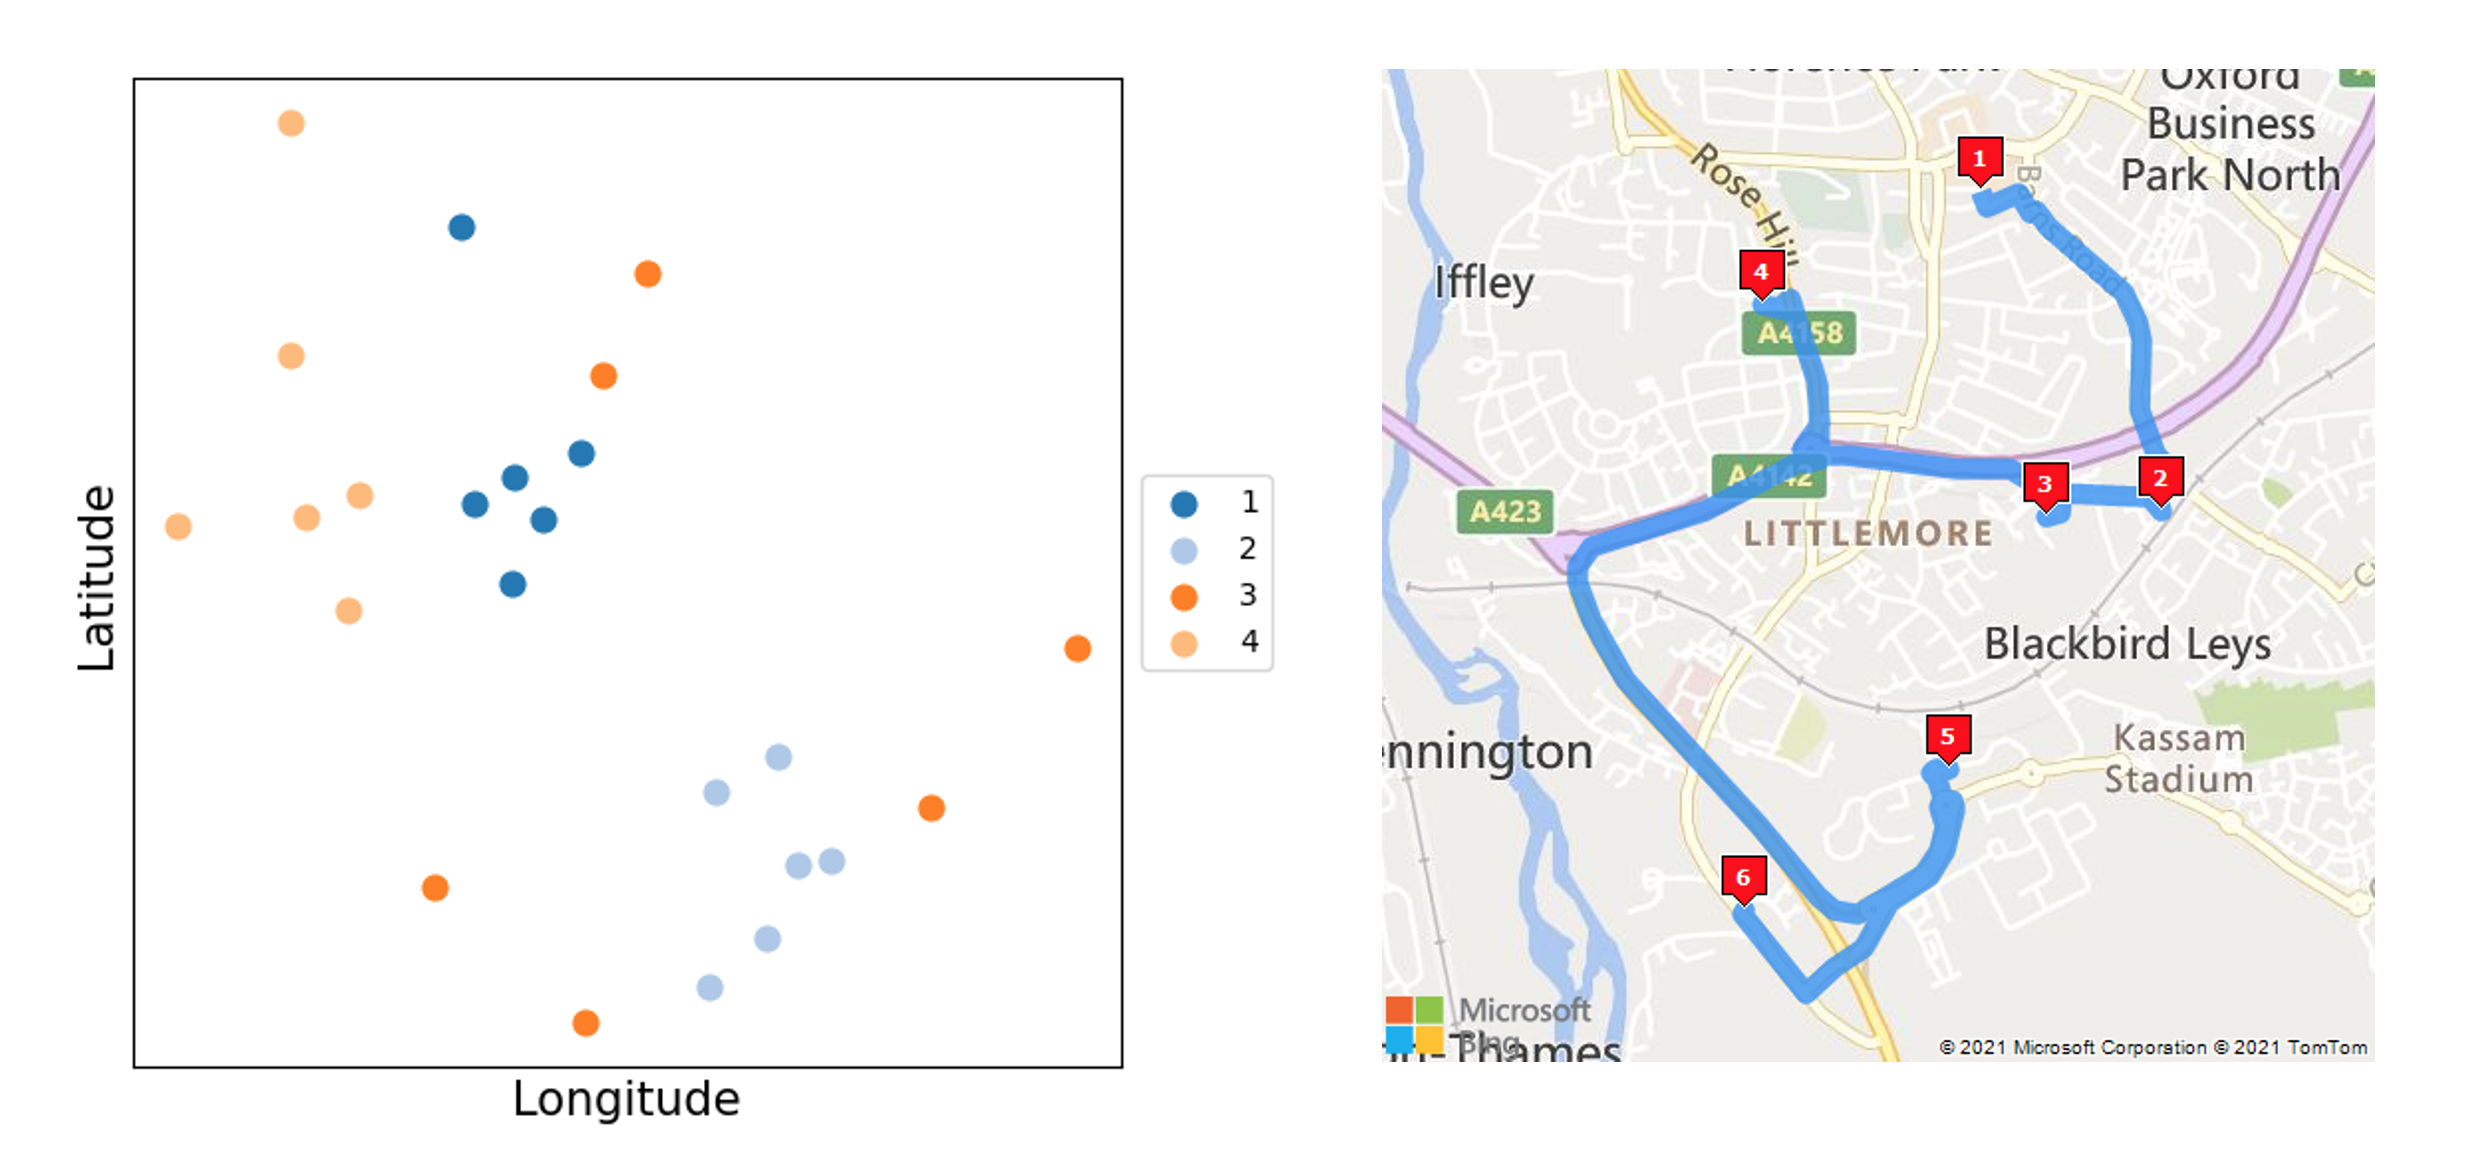
\includegraphics[width=\textwidth]{demo.png}
\caption{Example output produced by \vm{}. Left: 24 patients have been sorted into three clusters of size eight, the spatial distribution of which is shown here. Right: the optimal driving route for visiting the patients in cluster no. 2 (dark blue).}
\label{demo}
\end{figure}

The purpose of this paper is threefold. First, to highlight the rapid deployment of a free digital technology to meet time-sensitive vaccination requirements. Secondly, to explain how the service functions and, finally, to estimate the benefits arising from its use thus far (via time savings in vaccine delivery). This article is of interest to those involved in the development and implementation of digital technology into the health service, and the planning or delivery of services to housebound patients, be they vaccination-related or otherwise.

\section{Methods \& Materials}
\subsection{Implementation}

In this work, the term \textit{housebound} is used to refer to any individual whose postcode was uploaded to the Vaximap site for the purpose of planning a vaccination. Due to the anonymous nature of the tool, it is not possible to know on what medical basis they are deemed housebound. 

The problem is posed as finding the shortest routes to visit a set of $N$ patients, whilst ensuring any individual practitioner visits no more than $D$ patients on a route. It is assumed, but not required, that $D$ is set as the number of vaccine doses in a vial (for example, nine for Oxford-AstraZeneca); any number between 3 and 25 inclusive can be used. It follows that the $N$ patients must be sorted into $G = \mathrm{ceiling}(N/D)$ groups (rounded up in the case that $D$ does not divide perfectly into $N$, in which case \textit{exactly} one group will have size less than $D$)\footnote{This is an important extra constraint added at the request of a GP, which ensures at most one vial of vaccine will be incompletely consumed.}. 

Patient postcodes uploaded by the user are transformed into latitude and longitude coordinates via the use of Microsoft Bing's geocoding service. Patients are then grouped so that they are proximal in space according to Euclidean distance, a simple heuristic to minimise the travel time within each group. Iterative $k$-means clustering is used to group the patients subject to the constraint on group size $D$, which standard $k$-means cannot do \cite{macqueen1967some, davidson2005clustering}. Qualitatively, this approach prioritises those patients that are far away from all others to ensure they are assigned to their optimal group first, whereas those that are close to the centre of the distribution can be assigned last to any group with limited impact on the optimality of the routes. The clustering process is illustrated in figure \ref{clustering}. 

\begin{figure}[H]
\centering
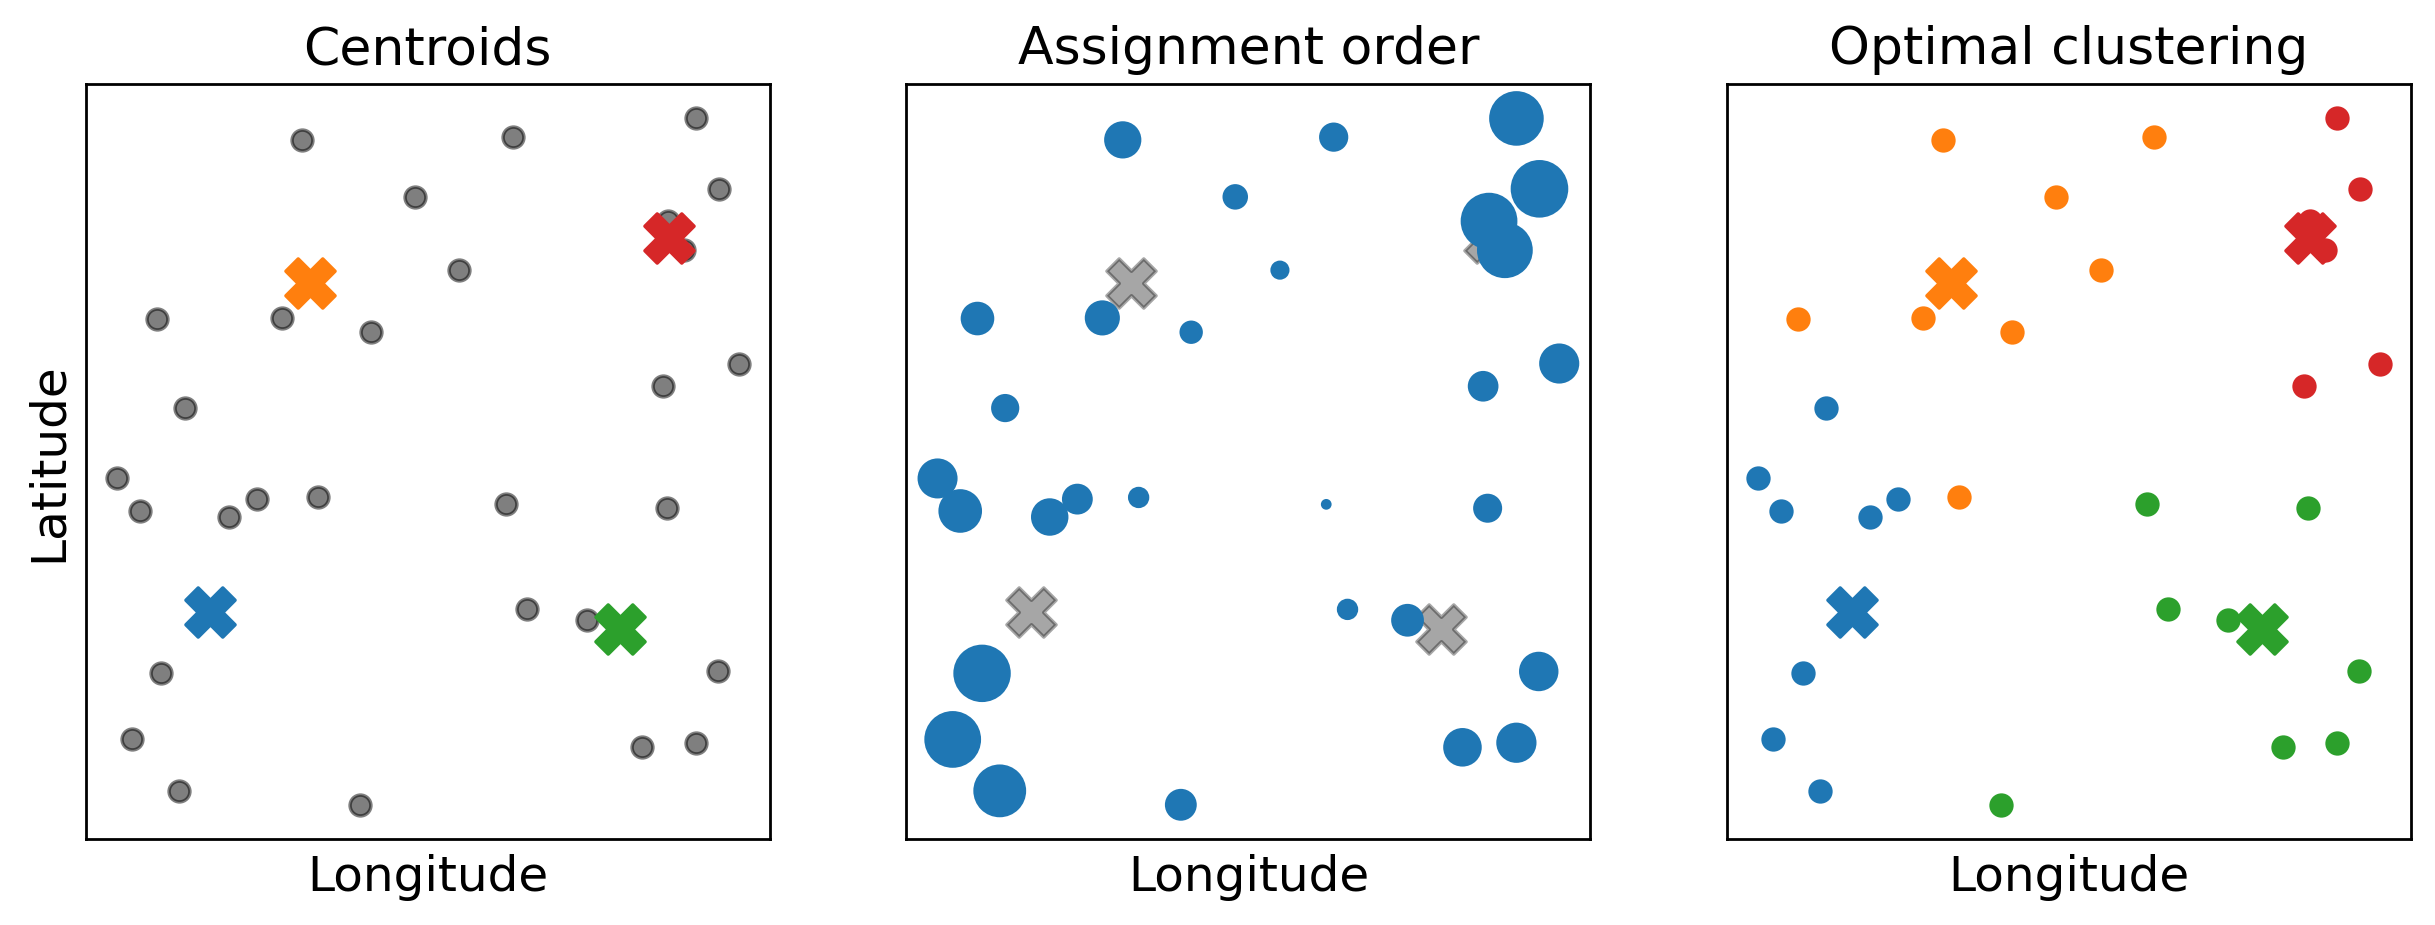
\includegraphics[width=\textwidth]{clustering_demo.png}
\caption{Example clustering of $N$ = 30 patients into groups of $D$ = 8. Left: initialisation of four cluster centroids (denoted with crosses). Centre: order of patient assignment, where larger circles indicate priority assignment and will be dealt with first. Patients in the centre of the distribution could be assigned to any cluster with low cost, so are dealt with last. Right: the optimal clustering of patients after assignment. The red cluster has six patients due to imperfect number division, whereas all other clusters are fully-sized.}
\label{clustering}
\end{figure}

After cluster assignment, the final step is to determine the optimal order in which to visit the patients of each group. This is achieved via Microsoft Bing’s mapping API, making use of the \textit{optimise waypoints} facility (which imposes a limit of 25 patients per group) \cite{msbing}. Optionally, the user can specify a fixed start and end point for their routes (for example, the address of their GP surgery); each route will then be a round-trip from that location. The user is returned the patient groups, the optimal driving or walking directions to visit each group, and travel time estimates. 

\subsection{Dataset}

Since the launch of the \vm{} service in January 2021, a database of service usage has been accumulated (in accordance with the website's privacy policy). From each user \textit{request} (corresponding to a single upload of patient postcodes and the routes that result), the following data are retained: time and date; number of patients; requested cluster size; relative distances between patients (not absolute locations); and transport mode. For approximately half of requests, counts of patient postal districts\footnote{Typical postal districts have in excess of 10,000 patients \cite{OfficeforNationalStatistics}, so this information is geographically non-precise.} were also retained (this is the first part of a postcode, for example OX1). As of May 2022, the dataset comprises approximately 13,000 requests for 395,000 patients; postal district information is available for 6,600 of the requests.


\subsection{Analysis methods}

The objective of analysis was to estimate the time savings yielded by \vm{} and to identify high-level trends in how the service has been used. The savings arise in two ways: firstly, when \textit{planning} a route to visit patients; and secondly when \textit{following} an optimal route instead of a sub-optimal one. The following analyses were performed. 

\paragraph{Repeat detection}
 In the course of development, it was noted that users sometimes uploaded the same set of patients multiple times in quick succession, with slightly different parameters. It is suspected that such behaviour reflects a learning process on the part of users who were familiarising themselves with the site. For some of the analyses detailed below, such repeat requests (defined by creation less than 21 days after a previous identical request) were removed. It was not desired to remove repeats separated by more than 21 days as these could represent genuine repeat uses, though they may not correspond to repeat vaccinations if separated by just a few weeks.

\paragraph{Summary metrics}
Summary metrics of the dataset were explored by drawing histograms of the number of patients uploaded per request, the number of clusters the request was split into, and the number of patients per cluster. The time-series nature of the data was explored by plotting the number of user requests per day, and the total number of patients across all requests per day. Finally, the geographic distribution of the data was exploited by plotting the cumulative number of patients across all requests in each UK postal district for the subset of data with this information. These analyses were performed on the dataset including repeats.

\paragraph{Savings in route planning}
The time taken for humans to plan solutions for the TSP is remarkably quick and scales linearly with the number of locations to be visited \cite{Macgregor1996, Dry2006, MacGregor2011}. The problem solved by \vm{} is subtly different to the conventional TSP investigated in the literature because users start with a text-based list of addresses (\textit{i.e}, from an EMIS database) as opposed to a visual representation. This difference is important in light of the consensus view that ``humans require a visual representation of the problem'' in order to solve it effectively \cite{MacGregor2011}. The time taken to plan routes in the absence of \vm{} can therefore be split into two components: a \textit{lookup time} to generate a spatial representation of the problem, and a \textit{routing time} to actually plan the routes using this representation.

A survey that investigated these components separately was conducted across 20 volunteers (8 female, 12 male, mean age 45 years). To estimate lookup time, respondents were asked to identify on a map the location of 5, 8 and 12 sites (identified by their postcodes). To estimate routing time, respondents were asked to propose the optimal route to visit 13, 20 and 26 pre-labelled sites in 2, 3 and 4 routes respectively, where no individual route could exceed 7 sites (which represents the constraint of a fixed group size). Linear regression of the completion times yielded the following estimates for the time taken to perform these tasks manually: 36.4 seconds/location for lookup time, and 4.8 seconds/location for planning time (uncertainties are quantified in the supplementary material). Thus, for a 5-site route, we would expect 182 seconds of lookup time, and 24 seconds of planning time, totalling 206 seconds.

The determined coefficients were then multiplied across the entire dataset, including repeats, to obtain estimates of the time saved in planning. Repeats were included in this analysis as it was assumed users had reasonable cause for them (for example, experimenting with different cluster sizes and observing the differing travel times that result before making a decision).

\paragraph{Savings in route following}
The quality of human solutions to the TSP has been investigated extensively \cite{Macgregor1996, MacGregor2011, Vickers2001, MacGregor1999a}. These are often remarkably close to optimal for small problems and scale well  for larger problems ($n > $ 50 locations). The empirical model of performance given in figure 2b of Dry's review \cite{Dry2006}, reproduced below in figure \ref{dry_model}, was used in this work to approximate the extra distance penalty $p(n)$ of human solutions compared to \vm{}'s solution. The penalty is very small for problems with $n \leq$ 25 patients. For each user request in the non-repeated dataset, the total (closed) length of the \vm{} generated routes $L_{vm}$ was calculated using the method given in the supplementary material. The approximate length of the human solution $L_h$ to the same problem was then obtained by multiplication with a scaling factor of $(1 + p(n))$ drawn from figure \ref{dry_model}. In order to convert distance savings into time savings, a mean driving speed of 50 km/h or 30 mph was assumed \cite{Balendra2020}. Repeats were not included in this estimate as it was assumed to be unlikely that the journeys themselves were undertaken (though a user may have planned the same route twice in a week, they are unlikely to have actually undertaken it twice).  

\begin{figure}[H]
\centering
\includegraphics[width=0.6\textwidth]{dry_model.png}
\caption{An empirical model of human performance on the TSP, taken from Dry's review \cite{Dry2006}. The individual observations from that work are reproduced here; a curve fit of the form $A(1 - e^{n/B})$ was performed to yield a smooth model. The penalty is less than 10\% for problems sized up to around 60 locations.}
\label{dry_model}
\end{figure}

\section{Results}

\paragraph{Summary metrics}
\begin{figure}[H]
\centering
\includegraphics[width=\textwidth]{timeseries.png}
\caption{Time series of Vaximap use. Peaks assumed to correspond to the majority of first (Jan `21) and second doses (Apr `21) can be discerned, as can booster doses (Nov  `21 and May `22). The red line is the 30-day moving average of total uploaded patients per day. A few uploads of the maximum permitted number of patients (300 patients) can be observed.}
\label{timeseries}
\end{figure}

Figure \ref{timeseries} shows the time series of Vaximap use cases, both in terms of total number of daily patients, and patients per user request. We note four peaks: February, April and November in 2021, and May 2022, which correspond to the first, second and booster vaccination doses in the UK.

\begin{figure}[H]
\centering
\includegraphics[width=0.7\textwidth]{postcodes.png}
\caption{Distribution of processed patient locations within UK postal districts, for a subset of the complete datset. Grey denotes no data.}
\label{uk_overview}
\end{figure}

Figure \ref{uk_overview} shows the geographic distribution of uploaded patient locations within the UK, for a subset of the complete dataset. Use of the service has been concentrated in England and Wales; by contrast Scotland has seen very little use.  

\begin{figure}[H]
\centering
\includegraphics[width=\textwidth]{hists.png}
\caption{Histograms of user request characteristics. Left: total number of patients uploaded. Centre: request cluster size. Right: number of clusters per request.}
\label{hists}
\end{figure}

Figure \ref{hists} shows summary statistics of uploaded user requests. Users uploaded a median of 17 and mean of 30 patients per request, with a target cluster size of around 10. Though a handful of users uploaded the maximum limit of 300 patients, a substantial minority uploaded 10 or so patients, resulting in a single cluster being generated. 

\paragraph{Repeat detection}
Using a 21 day repeat threshold, 3,666 repeat requests were detected. After excluding repeats, the dataset was reduced from 12,938 requests covering 393,186 patients to 9,272 requests covering 256,903 patients. The latter figure represents the best estimate of the number of actual, not potential, home visits that have been performed using the service. 

\paragraph{Time savings in route planning}
Applied to the full dataset including repeats, the survey-derived lookup times and routing times of 36.4s and 4.8s per location, respectively, yielded an estimate of total time savings in planning of 4,499 hours, equivalent to 112 weeks at 40 hours/week. 

\paragraph{Time savings in route following}
Applied to the full dataset without repeats, an empirical model of human performance on the TSP yielded an estimate of the total savings in distance travelled of 40,374 km. This is equivalent to 807 hours, or 20 weeks at 40 hours/week, assuming a mean travel speed of 50 km/h or 30 mph.

Combining all savings together yielded a total of 5,307 hours of practitioner time, equivalent to 132 work-weeks or 2.75 work-years. The time savings break down approximately in a 4:1 ratio for planning to travelling. Using mean salary estimates of £38,000 and £32,000 for a practice manager and community nurse respectively\footnote{Taken from \hyperlink{www.glassdoor.com}{www.glassdoor.com}}, these time savings can be converted into a cost saving of approximately £102,000. 

\section{Discussion}

We have presented a simple and easy-to-use solution for optimising vaccine delivery to housebound patients. It has seen widespread use during the UK's Covid-19 vaccination campaign, reaching 50\% of the target patient population\footnote{Assuming a patient population of 500,000 and using a figure of 250,000 non-repeated visits planned on the site.}, and yielded both time (close to three years of practitioner time) and cost (approximately £102,000) savings. One user in Plymouth reported doubling their rate of delivery through using the service, demonstrating that \vm{} was able to reduce the burden on the healthcare system both in simplifying the execution of a complex task, and also by quickly removing vulnerable patients from the unvaccinated population. In turn, the time savings obtained allowed primary care staff to focus on their other care responsibilities. 

Harder to quantify are the savings in cognitive load of automating the complicated process of route planning, but direct feedback from users (published on the \vm{} website) frequently touched on the `frustration' inherent to such a tedious and labour-intensive task. This is especially relevant given the small number of users that uploaded requests containing the maximum allowed number of 300 patients; manually planning for this number would be infeasible. These large requests also serve to illustrate the unequal demand for, and provision of, primary care to housebound patients across the country \cite{Rolewicz2021}: a GP surgery looking after hundreds of such patients faces very different challenges to one looking after a few dozen. In light of the very low investment that was required to set up this service (the beta version was online in 48 hours), the overall cost-benefit ratio of this solution is extremely favourable. 

The development of \vm{} relied upon real-time feedback from users. For example, the addition of walking directions (alongside driving) was made in response to requests from GP surgeries in urban areas. Widespread adoption was achieved almost entirely through word of mouth (in particular, GP networks on social media) with no engagement from the NHS itself. This shows the importance of interacting directly with users before and during development to ensure their requirements are met, which is pertinent in light of the expectation that digital technologies will play an ever-greater role in primary care \cite{WorldHealthOrganizationWHO2018}. 

At the time of writing, the service is supporting ongoing booster campaigns, as evidenced by the successive waves shown in figure \ref{timeseries}. Given the decay of protection afforded by the vaccine as time passes, and the emergence of new variants, \vm{} is well placed to assist with future Covid vaccination efforts. More importantly, the underlying problem that the service addresses will continue to exist long after Covid-19; namely, how to efficiently visit a set of patients subject to some constraint on group size? The technology could therefore be applied in other domains. An obvious example, and one already suggested by multiple users, would be supporting annual flu vaccination campaigns; a more novel example would be supporting district nurses, community nurses and physiotherapists in their daily tasks. Given that community healthcare in the UK records around 100 million patient contacts annually with a budget of around £10 billion and one-fifth of the NHS workforce \cite{Fund2019}, the cumulative impact of efficiencies obtained at the grassroots level could be substantial. 

\section{Contributions}

TFK developed the \vm{} software and website, and set up data collection. RS identified the core need, found a community of beta testers, and acted as clinical liaison for users throughout. AJB and AB performed survey and data analysis. All authors prepared and approved the manuscript. TFK, AJB and AB verified the data. All authors had access to the data and accompanying analysis. AJB, AB and RS were acting independently of their respective employers; this work has not been endorsed by, nor does it reflect the views of, Squarepoint Capital LLP, Vodafone Group PLC, Defence Medical Services or the Ministry of Defence. 

\section{Conflicts of interest}

TK, RS and Oxford University Innovation are shareholders in Vaxine Limited, a registered company in England and Wales (number 13182914), which owns the intellectual property of Vaximap. The authors declare no other conflicts of interest. 

\section{Acknowledgements}

The authors acknowledge financial support provided by Magdalen College, Oxford, Oxford University Innovation, and JHubMed, part of UK Strategic Command. Support of a technical nature was provided by Microsoft Bing. The authors thank Dr David Andrews for valuable feedback during the development of the service, and Captain Amrit Sandhu for integrating support from JHubMed. 

\section{Data access}

The authors intend to make the \vm{} dataset freely available following peer review. This will be via insertion into the Oxford Research Archive with accompanying DOI. The source code used for analysis of the dataset will also be released on GitHub. Until such a time, readers should contact the corresponding author for all enquiries. 


\bibliographystyle{unsrtnat}
\bibliography{../../../Documents/library.bib}

\end{document}